\documentclass{article}

\usepackage{amsmath,amssymb,amsfonts}
\usepackage{listings}
\usepackage{graphicx}
\usepackage{textcomp}
\usepackage{xcolor}
\usepackage{multirow}
\usepackage{booktabs}
\usepackage{hyperref}
\usepackage{afterpage}
\usepackage{float}

\definecolor{lstgray98}{rgb}{0.98,0.98,0.98}
\definecolor{bashbg}{rgb}{0.93,0.95,0.97}

\graphicspath{{Images/}}

\lstdefinelanguage{json}{
  basicstyle=\ttfamily\small,
  showstringspaces=false,
  breaklines=true,
  frame=single,
  literate=
   *{0}{{{\color{blue}0}}}{1}
    {1}{{{\color{blue}1}}}{1}
    {2}{{{\color{blue}2}}}{1}
    {3}{{{\color{blue}3}}}{1}
    {4}{{{\color{blue}4}}}{1}
    {5}{{{\color{blue}5}}}{1}
    {6}{{{\color{blue}6}}}{1}
    {7}{{{\color{blue}7}}}{1}
    {8}{{{\color{blue}8}}}{1}
    {9}{{{\color{blue}9}}}{1}
}

\lstdefinestyle{mamstyle}{%
    language=C,
    float=tb!,
    floatplacement=tb!,
    basicstyle=\scriptsize,
    columns=fixed,
    showstringspaces=false,
    extendedchars=false,
    breaklines=true,
    breakatwhitespace=true,
    breakindent=1em,
    frame=single,
    showtabs=false,
    showspaces=false,
    identifierstyle=\ttfamily,
    keywordstyle=\color[rgb]{0,0,1},
    stringstyle=\color[rgb]{0.627,0.126,0.941},
    backgroundcolor=\color{lstgray98},
    captionpos=b,
    escapechar=§,
    aboveskip=0pt,
    belowskip=0pt,
    xleftmargin=0.7cm
}

\lstdefinestyle{bashstyle}{%
    language=bash,
    basicstyle=\ttfamily\small,
    columns=fullflexible,
    showstringspaces=false,
    breaklines=true,
    frame=single,
    numbers=none,
    backgroundcolor=\color{bashbg},
    captionpos=b,
    aboveskip=0.5em,
    belowskip=0.5em
}

\lstset{
  basicstyle=\fontsize{9}{11}\selectfont\ttfamily,
  breaklines=true,
  columns=fullflexible,
  keepspaces=true
}

\begin{document}

\title{Proteo User Manual\\
\large Configurable Synthetic Application for Studying Malleability in HPC}

\author{}
\date{\today}

\maketitle

\tableofcontents
\newpage

\section*{Quick Install}
\addcontentsline{toc}{section}{Quick Install}

This page summarizes the shortest path from clone to a first run. See Section~\ref{section:installation} for prerequisites and build options.

\begin{lstlisting}[style=bashstyle,caption={Minimal Proteo setup and smoke test.},captionpos=b]
git clone http://lorca.act.uji.es/gitlab/martini/malleability_benchmark.git
cd malleability_benchmark

cd Codes
make MAM_USE_SLURM=1

cd ../Results
bash ../Exec/singleRun.sh ../Codes/test.json mypartition 0 1 0
\end{lstlisting}

Replace \texttt{mypartition} with a valid Slurm partition. On success, output files such as \texttt{R0\_Global.out} appear in the current directory.

\begin{itemize}
  \item JSON parameter reference: Section~\ref{section:json-config}
  \item Web editor for JSON files: Section~\ref{section:genconfig}
  \item Execution scripts and outputs: Section~\ref{section:usage}
\end{itemize}

\section{Introduction}
\label{section:introduction}

\textbf{Proteo} is a configurable synthetic application for studying \textit{malleability} in high-performance computing (HPC). It emulates the behaviour of iterative MPI scientific applications that can be resized on-the-fly (expanded, shrunk, or migrated) while running under a resource manager.

Proteo is composed of two C/MPI modules:

\begin{itemize}
  \item \textbf{SAM} (Synthetic Application Module): emulates application \textbf{computation}, \textbf{communication}, and \textbf{I/O} through configurable \textit{phases} and \textit{stages}.
  \item \textbf{MaM} (Malleability Module): performs dynamic process management, spawn/shrink operations, and data redistribution between source and target process groups.
\end{itemize}

Proteo focuses on \textbf{iterative MPI applications} whose iterations combine compute, MPI communication, and I/O stages. With the appropriate JSON configuration, it can approximate a wide range of MPI application profiles.

\subsection{Terminology}

During a resize operation, the existing process group is referred to as \textit{sources}; the newly created group is the \textit{targets}. Depending on the spawn method and strategy, some source ranks may also join the target group. In all cases, the target group continues the emulated application execution.

A \textbf{phase} is a segment of the emulated application: it runs for a fixed number of iterations (\texttt{Total\_Iters}) and contains an ordered list of \textbf{stages} (computation, MPI communication, or I/O). Phases are executed sequentially within a process group.

A \textbf{group} defines one segment of the overall malleable execution: how many MPI processes run, for how many iterations, and which MaM spawn/redistribution options apply before the next resize (if any). The number of groups is \texttt{Total\_Resizes}~$+~1$.

\subsection{Configuration format}

Proteo is configured through \textbf{JSON files}. Each file describes:

\begin{enumerate}
  \item Global simulation parameters (\texttt{general}).
  \item One or more application phases with nested stages (\texttt{phases}).
  \item One process group per resize boundary (\texttt{groups}).
\end{enumerate}

The web tool \textbf{GenConfig} (Section~\ref{section:genconfig}) helps create and validate these files. Section~\ref{section:json-config} documents every parameter.

\subsection{Manual organization}

\begin{itemize}
  \item Section~\ref{section:architecture}: SAM/MaM architecture and execution model.
  \item Section~\ref{section:installation}: prerequisites and build instructions.
  \item Section~\ref{section:usage}: execution scripts and output files.
  \item Section~\ref{section:json-config}: JSON parameter reference.
  \item Section~\ref{section:genconfig}: GenConfig web editor and combinatorial expansion.
  \item Section~\ref{section:examples}: worked examples.
  \item Section~\ref{section:analysis}: post-run analysis.
  \item Appendix~\ref{appendix:csv}: CSV output format for custom analysis.
\end{itemize}

\section{Architecture}
\label{section:architecture}

Proteo emulates a malleable MPI application through five cooperating modules inside SAM, backed by MaM for resize operations.

\subsection{SAM modules}
\label{subsection:sam-modules}

\begin{enumerate}
  \item \textbf{Initialization}: Rank~0 of the first group reads the JSON configuration from disk and builds the in-memory \texttt{configuration} structure. That structure is broadcast to every rank in the group and, after each resize, from the source root to target ranks. During initialization SAM also calibrates derived parameters (per-stage operation counts, communication volumes, I/O sizes) from the JSON values and the hardware where the job runs. This module runs once at job start and again for each target group after spawn and data redistribution.

  \item \textbf{Application emulation}: SAM executes the configured \textbf{phases} in order. For each phase it repeats \texttt{Total\_Iters} iterations; within each iteration every \textbf{stage} runs sequentially. Stages may emulate CPU-bound or memory-bound computation, blocking or non-blocking MPI communication, or parallel I/O. Timings are recorded per stage and per iteration for later output.

  \item \textbf{Resize}: When a non-final group completes its allotted work, MaM is invoked to spawn or merge target processes and redistribute application state from sources to targets. Depending on spawn strategy, sources may continue executing iterations while spawn or asynchronous redistribution proceeds in the background.

  \item \textbf{Monitoring}\label{subsection:monitoring}: Every stage, iteration, spawn, and redistribution interval is measured with \texttt{MPI\_Wtime}. Optional barriers (JSON \texttt{Rigid} and compile-time \texttt{MAM\_USE\_BARRIERS}) tighten timing accuracy at the cost of overhead.

  \item \textbf{Completion}: When a group finishes its role in the emulation, SAM writes intermediate result files containing configuration echo, per-stage timings, and malleability metrics ($T_{spawn}$, $T_{SR}$, $T_{AR}$, etc.).
\end{enumerate}

Figure~\ref{fig:flowchart} shows the overall control flow. Listing~\ref{code:basic-struct2} sketches the corresponding program structure.

\begin{figure}[htbp]
  \centering
  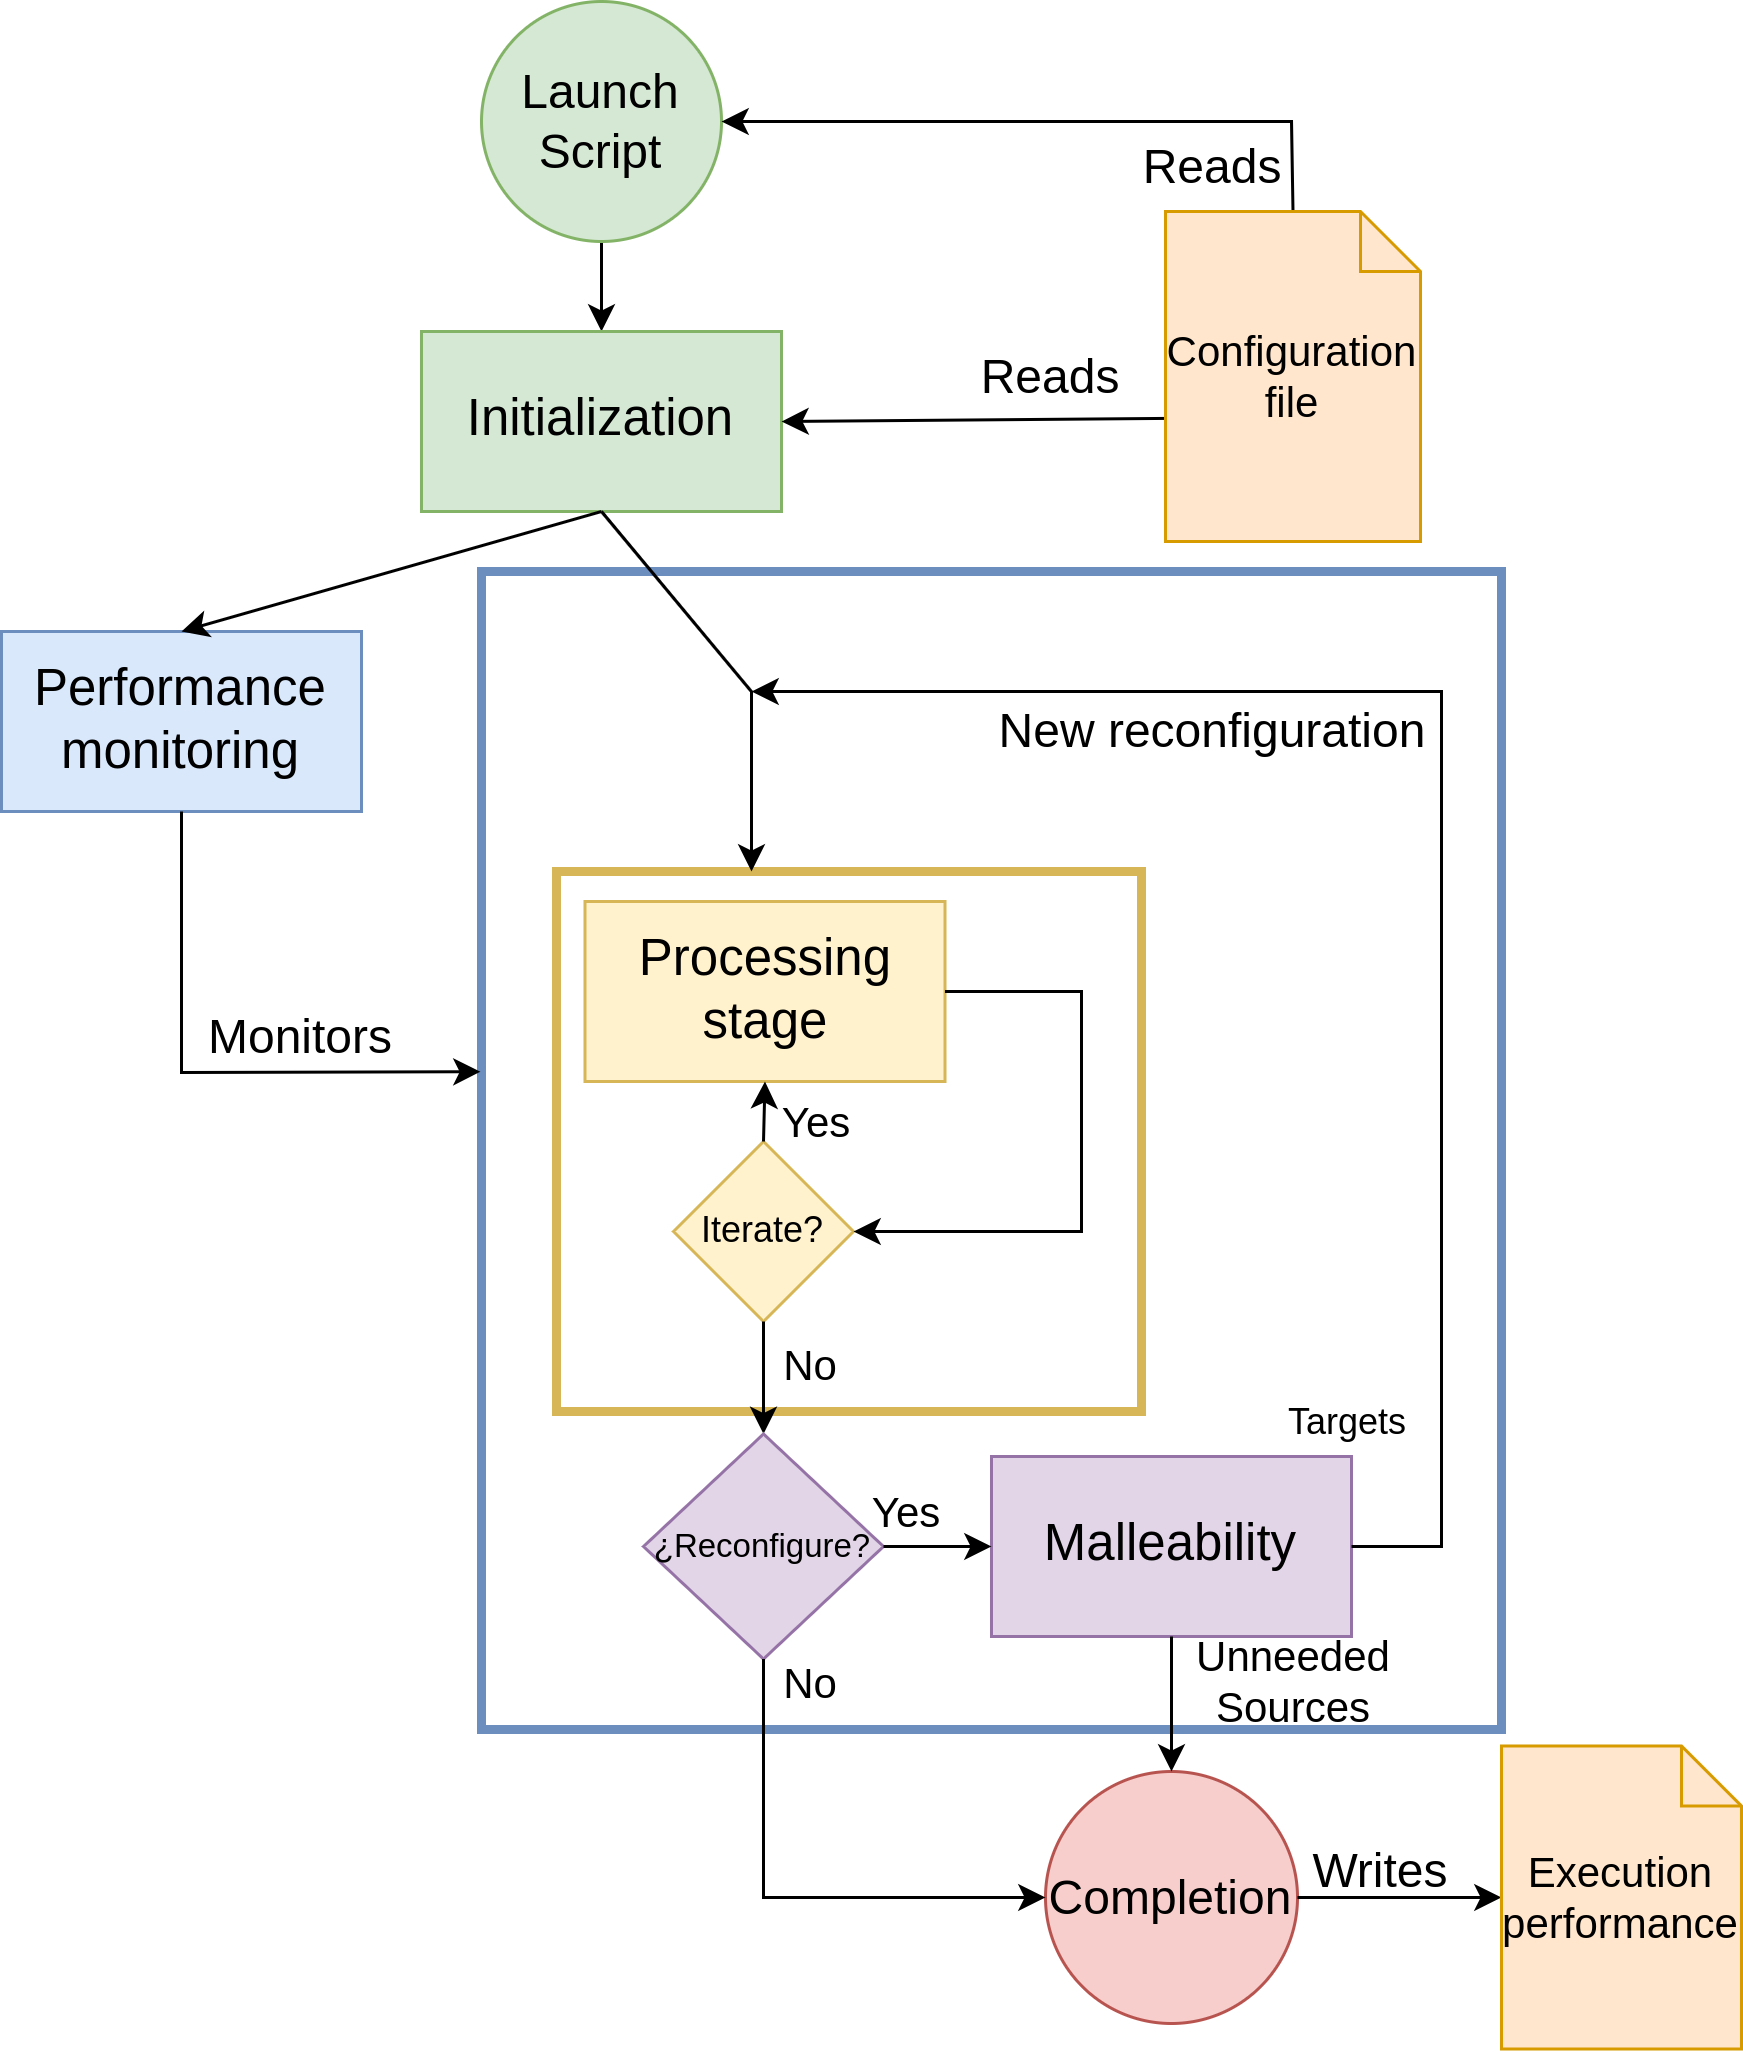
\includegraphics[width=0.85\textwidth]{NewFig1-EstructApp.jpeg}
  \caption{Flowchart of the synthetic application modules.}
  \label{fig:flowchart}
\end{figure}

\begin{figure}[htbp]
  \centering
  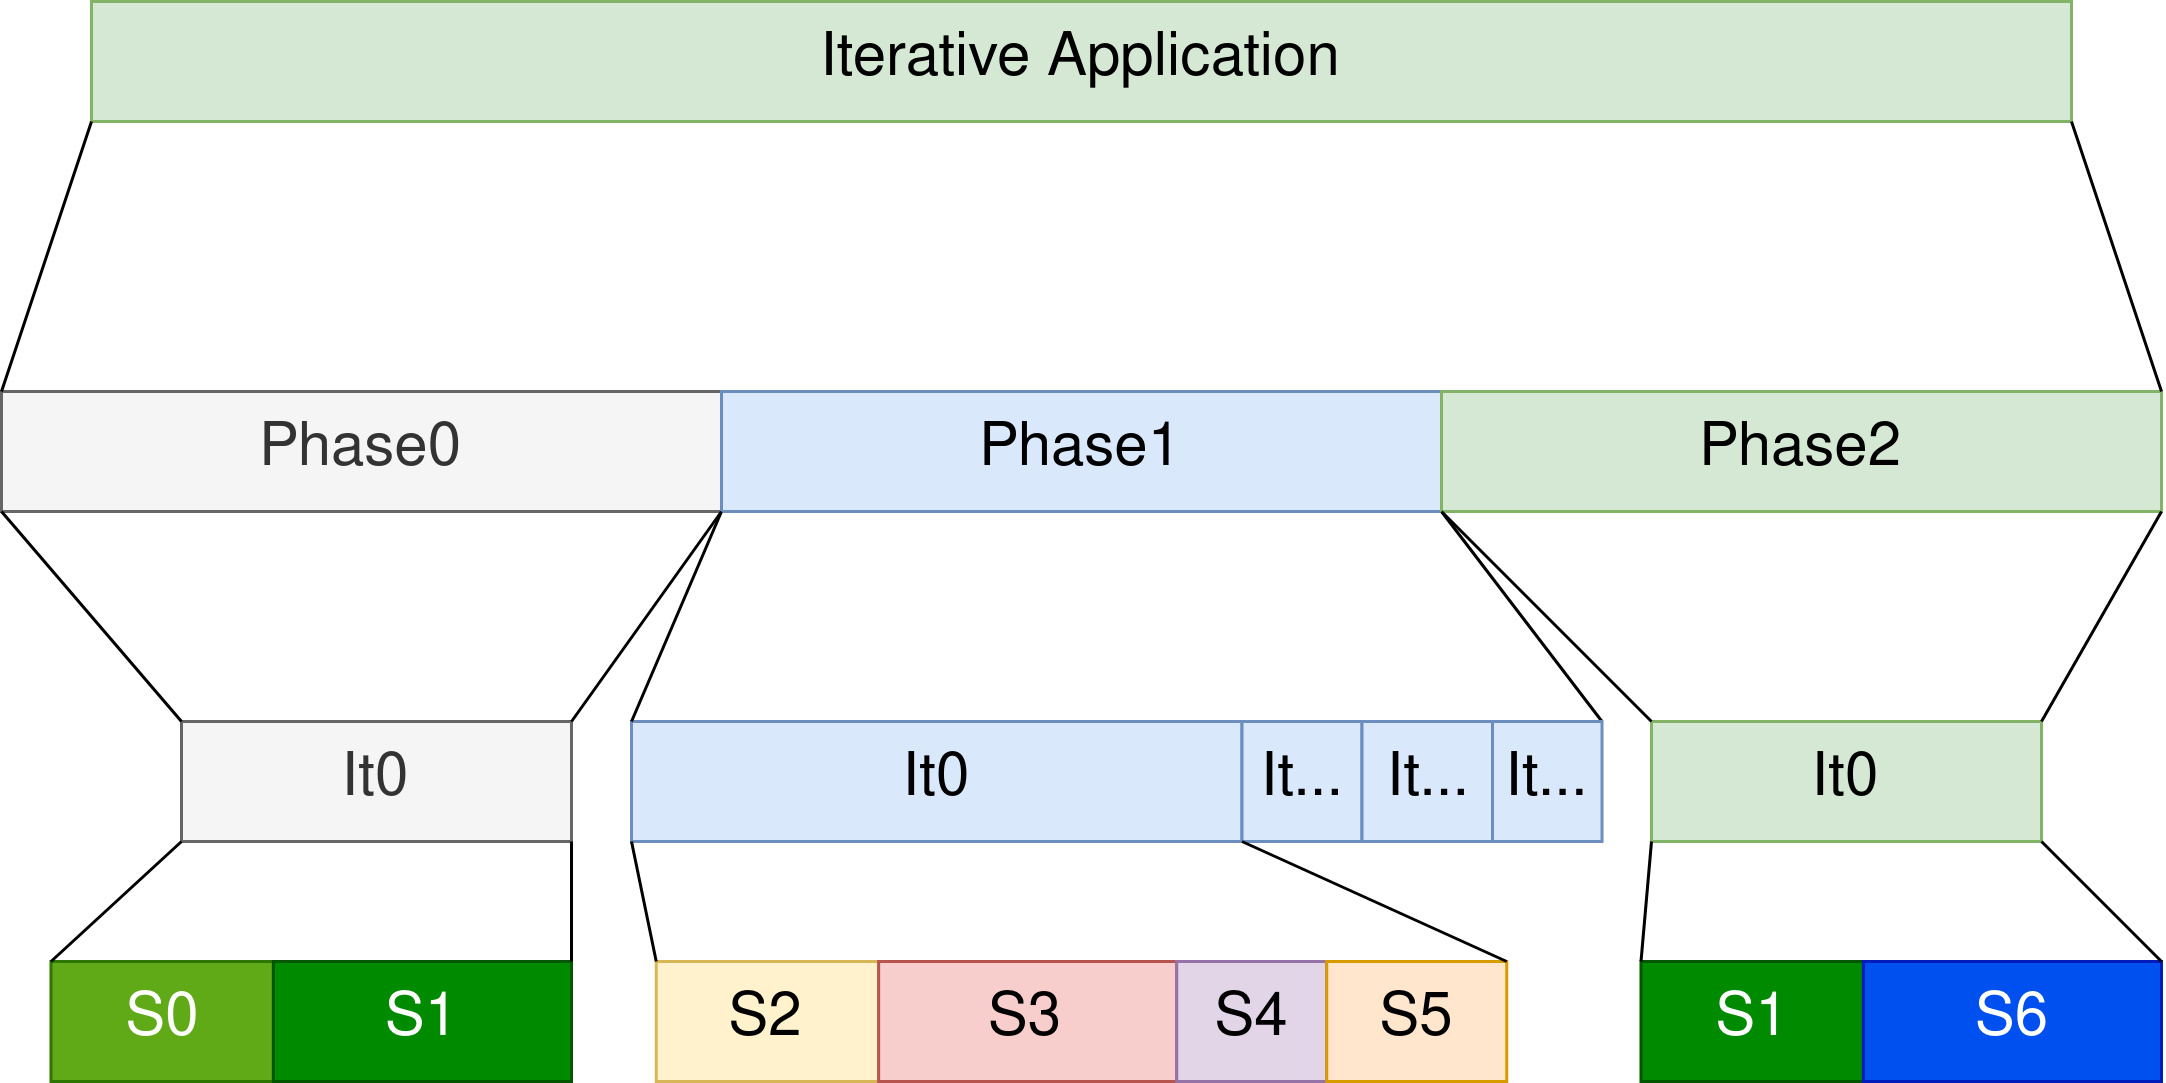
\includegraphics[width=0.75\textwidth]{Fig2-PhaseBasedIter.png}
  \caption{Phase-based iteration model: each phase defines its own stage sequence and iteration count.}
  \label{fig:phase-model}
\end{figure}

Each \textbf{phase} contributes \texttt{Total\_Iters} iterations; within each iteration all \texttt{stages} of that phase execute sequentially. When all phases of a group finish, a resize occurs unless this is the last group (see Section~\ref{subsection:group-termination}).

\subsection{Computation stages}
\label{subsection:compute-stages}

Compute stages drive CPU or memory workload without MPI messaging:

\begin{itemize}
  \item \textbf{Type 0 (Monte Carlo $\pi$)}: Repeated pseudo-random sampling to estimate $\pi$. The kernel is CPU-bound and does not perform large memory traversals. \texttt{Granularity} controls the sample count per operation; SAM repeats operations until the configured \texttt{Stage\_Time} is reached under the current \texttt{FactorS} and process count.

  \item \textbf{Type 1 (matrix--vector)}: Column-major matrix--vector multiplication. The kernel is memory-bandwidth bound. As with type~0, \texttt{Granularity} sets the problem size and \texttt{Stage\_Time} sets the target duration after scaling.
\end{itemize}

For both types, \texttt{Stage\_Bytes} is unused. SAM derives an internal operation count from the measured baseline time $T_{op}$ at the current \texttt{Granularity}, the configured \texttt{Stage\_Time}, and the group \texttt{FactorS}. After a resize, $T_{op}$ and the operation count are recomputed if \texttt{FactorS} or \texttt{Procs} changes (Section~\ref{subsection:factors}).

\subsection{Communication stages}
\label{subsection:comm-stages}

Communication stages exercise MPI patterns among ranks in the active group:

\begin{itemize}
  \item \textbf{Point-to-point (2)}: \texttt{MPI\_Sendrecv} between ranks on neighbouring nodes following a ring-like neighbour assignment.
  \item \textbf{IPoint-to-point (3)}: Non-blocking send/receive posted with \texttt{Stage\_Identifier}. Must be paired with a Wait stage (type~4) that completes the outstanding requests.
  \item \textbf{MPI\_Wait (4)}: Completes non-blocking operations for a given \texttt{Stage\_Identifier}. One Wait stage may complete \textbf{multiple} IPoint stages that share the same identifier.
  \item \textbf{Bcast (5)}, \textbf{Allgather (6)}, \textbf{Reduce (7)}, \textbf{Allreduce (8)}: Standard MPI collectives over the group communicator.
\end{itemize}

Each communication stage must specify either \texttt{Stage\_Bytes}~$>$~0 (preferred: explicit message volume) or \texttt{Stage\_Time}~$>$~0 (timed emulation from which SAM derives bytes using network calibration). Non-compute granularity rules apply when bytes are absent or when time-capping is enabled; see Section~\ref{subsubsection:stage-validation}.

\subsection{I/O stages}
\label{subsection:io-stages}

\begin{itemize}
  \item \textbf{Write (9)} and \textbf{Read (10)}: Emulated parallel I/O. Each stage requires \texttt{Stage\_Bytes}~$>$~0 or \texttt{Stage\_Time}~$>$~0, plus \texttt{Stage\_Involved\_Procs} ($0$ means all ranks participate). These stages let Proteo model applications whose iterations include checkpointing, restart, or dataset movement alongside compute and MPI traffic.
\end{itemize}

\subsection{MaM resize pipeline}
\label{subsection:mam-resize}

A resize involves three steps:

\begin{enumerate}
  \item Signal availability to the resource manager (simulated via configuration when Slurm integration is enabled).
  \item Create the target MPI process group (\textit{spawn}).
  \item Redistribute data from sources to targets (\textit{redistribution}).
\end{enumerate}

\textbf{Spawn methods:}
\begin{itemize}
  \item \textbf{Baseline (0)}: Create $Y$ target processes and remove the $X$ sources (\texttt{MPI\_Spawn}).
  \item \textbf{Merge (1)}: Create or remove $|Y-X|$ processes and merge communicators where possible.
\end{itemize}

\textbf{Spawn strategies} (combinable indices in \texttt{Spawn\_Strategy}, except where noted):
\begin{itemize}
  \item \textbf{1 Pthread}: asynchronous spawn in a background thread.
  \item \textbf{2 Single}: only rank~0 spawns.
  \item \textbf{3 Intercomm}: intercommunicator-based spawn.
  \item \textbf{4 Multiple} / \textbf{5 Parallel}: multi-source strategies; \textbf{mutually exclusive} with each other. \textbf{Parallel} coordinates process creation with the RMS so expand and shrink operations keep allocations consistent with RMS rules (jobs do not violate resource-manager constraints when resizing).
\end{itemize}

\begin{figure}[htbp]
  \centering
  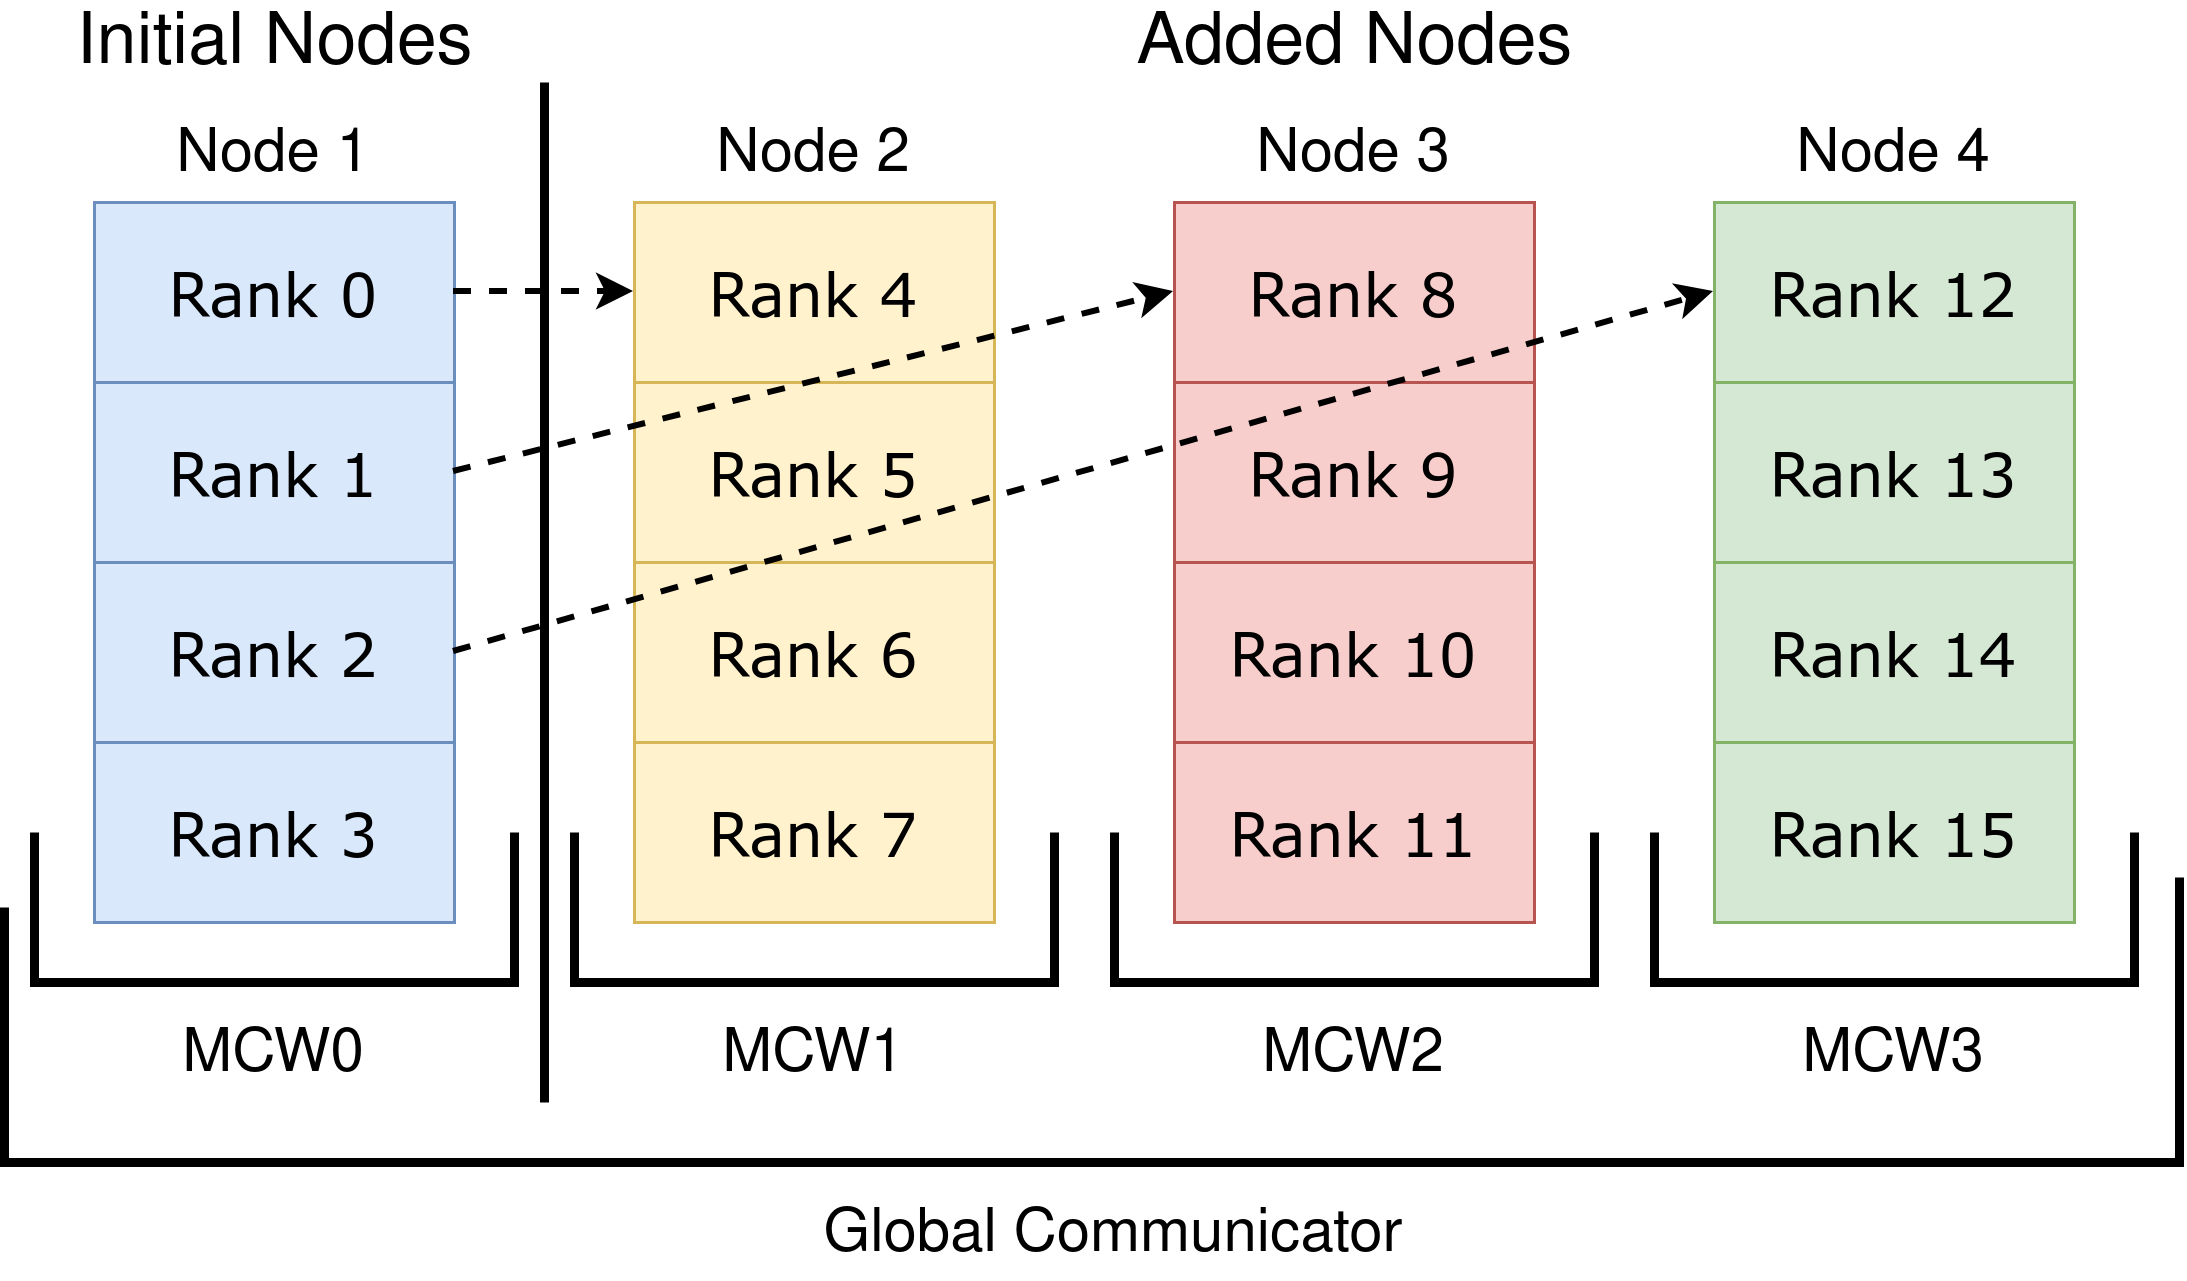
\includegraphics[width=0.85\textwidth]{Fig3-ParallelSpawn-Spawn-Poster.png}
  \caption{Overview of parallel spawn strategies in MaM.}
  \label{fig:parallel-spawn}
\end{figure}

\textbf{Physical mapping} (\texttt{Dist}):
\begin{itemize}
  \item \texttt{spread}: spread processes across as many nodes as possible.
  \item \texttt{compact}: fill nodes before using the next node.
\end{itemize}

\textbf{Data redistribution} splits the payload into synchronous (\texttt{SDR}) and asynchronous (\texttt{ADR}) \textbf{element counts}. The actual byte volume moved is \texttt{SDR}~$\times$~\texttt{Datasize} and \texttt{ADR}~$\times$~\texttt{Datasize}. Constant data may be sent asynchronously while sources continue computing; variable data is sent synchronously. Methods include all-to-all among sources (0), point-to-point (1), and RMA Lock / LockAll (2--3). Spawn and redistribution \textbf{strategy combination rules apply when ADR~$>$~0} (Section~\ref{subsubsection:strategy-rules}).

\subsection{General working}
\label{subsection:working}

Listing~\ref{code:basic-struct2} shows a simplified view of SAM's main control flow. Source ranks read and broadcast the configuration, then derive stage parameters. Target ranks receive the configuration from sources and complete data redistribution. All ranks then walk phases, iterations, and stages. If more groups remain, MaM spawns targets and redistributes state; otherwise the group writes its output files and finishes.

\begin{lstlisting}[style=mamstyle, numbers=none, float, caption={Basic skeleton of the synthetic application.}, label=code:basic-struct2, captionpos=b]
int main() {
  if (init) {
    if (rank == 0) read_config();
    broadcast_config();
    calculate_derived_parameters();
  } else {
    receive_config_from_sources();
    redistribute_data();
  }
  for (phase = 0; phase < n_phases; phase++)
    for (iter = 0; iter < phase_iters; iter++)
      for (stage = 0; stage < n_stages; stage++)
        process_stage(stages[stage]);
  if (!last_group) {
    spawn_targets();
    redistribute_data_to_targets();
  }
  write_output_files();
}
\end{lstlisting}

\subsection{FactorS and scalability}
\label{subsection:factors}

\texttt{FactorS} emulates how compute-stage duration scales with the process count. Values above~1 increase effective stage time; values below~1 decrease it. For an ideal speedup from 2 to 4 processes with sequential \texttt{Stage\_Time}~$=$~4~s, \texttt{FactorS} would be $0.5$ and $0.25$ respectively.

Non-direct parameters \texttt{$T_{op}$} (time per operation at current granularity) and \texttt{operations} (repeat count to reach the configured \texttt{Stage\_Time} under \texttt{FactorS}) are recomputed after each resize when \texttt{FactorS} changes.

\subsection{MaM as a standalone library}
\label{subsection:mam-library}

MaM can be linked into \textbf{other MPI applications} to add malleability (spawn, shrink, redistribution) without using SAM. Its public interface, configuration keys, and integration workflow will be documented in a \textbf{separate MaM manual}. This Proteo manual covers only the SAM+MaM benchmark path.

\section{Installation}
\label{section:installation}

This section describes how to obtain, compile, and verify a Proteo installation.

\subsection{Prerequisites}

\textbf{Required:}
\begin{itemize}
  \item GNU C compiler.
  \item \textbf{MPICH} 3.x or 4.0.x with OFI or Nemesis netmod. Dynamic process creation has been tested with MPICH. The UCX netmod has only been tested with MPICH~5.0.0.
  \item \textbf{Slurm} workload manager (tested with Slurm-wlm 19.05.5). Slurm is optional for compilation, but the default execution scripts assume it for job submission.
\end{itemize}

\textbf{Optional:}
\begin{itemize}
  \item Python~3.8+ with NumPy and Pandas (post-run analysis only).
  \item Flask (for GenConfig; see Section~\ref{section:genconfig}).
\end{itemize}

\subsection{Obtain the source}

Clone the repository:

\begin{lstlisting}[style=bashstyle,caption={Clone Proteo.},captionpos=b]
git clone http://lorca.act.uji.es/gitlab/martini/malleability_benchmark.git
cd malleability_benchmark
\end{lstlisting}

\subsection{Compile}

From the repository root, build with \texttt{make} in \texttt{Codes/}. Three optional flags control MaM behaviour (\texttt{Codes/Makefile}):

\begin{table}[H]
\centering
\small
\begin{tabular}{@{}llp{6.5cm}@{}}
\toprule
\textbf{Flag} & \textbf{Default} & \textbf{Meaning} \\
\midrule
\texttt{MAM\_USE\_SLURM} & 0 & Set to \texttt{1} to enable Slurm/RMS integration in MaM (required for normal Proteo runs with \texttt{singleRun.sh}). \\
\texttt{MAM\_USE\_BARRIERS} & 0 & Set to \texttt{1} to insert additional barriers inside MaM for stricter timing (may slow execution). Distinct from JSON \texttt{Rigid}. \\
\texttt{MAM\_DEBUG} & 0 & Debug verbosity at compile time; integer \texttt{0} (off) through \texttt{6} (most verbose). Values greater than~0 also enable compiler flags \texttt{-g} and \texttt{-O1}. \\
\bottomrule
\end{tabular}
\caption{MaM compile-time flags passed through \texttt{Codes/Makefile}.}
\end{table}

Typical Slurm-enabled build:

\begin{lstlisting}[style=bashstyle,caption={Build MaM and SAM with Slurm support.},captionpos=b]
cd Codes
make MAM_USE_SLURM=1
\end{lstlisting}

Optional debug or barrier build:

\begin{lstlisting}[style=bashstyle]
make MAM_USE_SLURM=1 MAM_USE_BARRIERS=1 MAM_DEBUG=3
\end{lstlisting}

This compiles the MaM shared library first, then links SAM (\texttt{Codes/SAM/build/a.out}). A configuration stub is written to \texttt{Codes/build/config.txt} and sourced by execution scripts.

To remove build artifacts:

\begin{lstlisting}[style=bashstyle]
cd Codes && make clean
\end{lstlisting}

\subsection{Repository layout}

\begin{itemize}
  \item \texttt{Codes/}: MaM and SAM source code and binaries.
  \item \texttt{Exec/}: Slurm launch scripts and Python helpers.
  \item \texttt{GenConfig/}: JSON configuration web editor.
  \item \texttt{Results/}: default directory for experiment outputs.
  \item \texttt{Analysis/}: Python scripts for post-processing.
\end{itemize}

\subsection{Verify the installation}

A minimal smoke test uses the sample JSON in \texttt{Codes/test.json}. From the directory where you want output files (e.g.\ \texttt{Results/}):

\begin{lstlisting}[style=bashstyle,caption={Smoke test with automatic Slurm allocation.},captionpos=b]
bash ../Exec/singleRun.sh ../Codes/test.json mypartition 0 1 0
\end{lstlisting}

Replace \texttt{mypartition} with a valid Slurm partition name on your system. On success, output files appear with names such as \texttt{R0\_Global.out}, \texttt{R0\_G0NP2.out}, and \texttt{slurm-*.out}.

Validate consistency with:

\begin{lstlisting}[style=bashstyle]
bash ../Exec/CheckRun.sh test 0 1 4 3 100
\end{lstlisting}

The script prints \texttt{SUCCESS} or \texttt{REPEATING} when runs are consistent; \texttt{FAILURE} indicates a configuration or build problem. Adjust \texttt{total\_stages} and \texttt{total\_groups} to match your configuration (see Section~\ref{section:usage}).

\section{Running Proteo}
\label{section:usage}

Proteo is launched through shell scripts in \texttt{Exec/}. All scripts accept \textbf{JSON} configuration files (extension \texttt{.json}). SAM selects the reader based on file extension.

\subsection{Single execution with automatic allocation}

\texttt{singleRun.sh} submits a Slurm job, computes the required node count from the JSON file, and runs the emulation.

\begin{lstlisting}[style=bashstyle,caption={singleRun.sh usage.},captionpos=b,label=code:singleRun-usage]
bash singleRun.sh config.json partition [outIndex] [repetitions]
                   [valgrind/extrae] [timeLimitSec] [outputDir]

bash singleRun.sh Codes/test.json mypartition 0 1 0
\end{lstlisting}

\begin{description}
  \item[\texttt{config.json}] Mandatory. Path to the JSON configuration.
  \item[\texttt{partition}] Mandatory. Slurm partition name.
  \item[\texttt{outIndex}] Optional (default~0). Prefix \texttt{R\{index\}} for output files.
  \item[\texttt{repetitions}] Optional (default~1). Number of runs with the same configuration.
  \item[\texttt{valgrind/extrae}] Optional (default~0). \texttt{0} = none, \texttt{1} = Valgrind, \texttt{2} = Extrae tracing.
  \item[\texttt{timeLimitSec}] Optional (default~0). Maximum time in \textbf{seconds} for a \textbf{single} execution. The script converts this to a Slurm wall-time limit as $(\texttt{timeLimitSec} \times \texttt{repetitions}) / 60 + 1$ minutes. \texttt{0} leaves the limit unset.
  \item[\texttt{outputDir}] Optional. Move \texttt{R\{index\}\_*} files to this directory after completion.
\end{description}

\subsection{Execution with singleRunCostum.sh}
\label{subsection:single-run-costum}

\texttt{singleRunCostum.sh} does \textbf{not} allocate resources itself. It launches Proteo with \texttt{mpirun} using the hosts available in the current environment. Parameters match \texttt{singleRun.sh} except there is no partition argument. Typical deployment modes:

\subsubsection{Local or personal computer}

On a single machine (no cluster), invoke the script directly after compiling. Without Slurm, the launcher falls back to the local hostname:

\begin{lstlisting}[style=bashstyle,caption={Local run without Slurm.},captionpos=b]
bash Exec/singleRunCostum.sh Codes/test.json 0 1 0
bash Exec/singleRunCostum.sh my_config.json 5 10 0 $HOME/results
\end{lstlisting}

This is the simplest way to try Proteo on a laptop or workstation.

\subsubsection{Cluster with Slurm}

Obtain an allocation first (\texttt{sbatch} or \texttt{srun}), then run the script \textbf{inside} that allocation so \texttt{SLURM\_JOB\_NODELIST} is set:

\begin{lstlisting}[style=bashstyle,caption={singleRunCostum.sh inside a Slurm allocation.},captionpos=b]
# Batch job that wraps the script
sbatch -N 2 -p mypartition --wrap \
  "bash Exec/singleRunCostum.sh Codes/test.json 0 1 0"

# Or interactively after srun / salloc:
bash Exec/singleRunCostum.sh Codes/test.json 0 1 0
\end{lstlisting}

\subsubsection{Multiple machines without an RMS}

When several hosts are available but no resource manager is used, MPI must be able to reach every machine (shared filesystem, SSH keys or equivalent). Either:

\begin{itemize}
  \item Export a comma-separated host list that the launcher can pass to \texttt{mpirun -hosts} (the script reads \texttt{SLURM\_JOB\_NODELIST} when set; without Slurm you can still export a host list in that variable), then call \texttt{singleRunCostum.sh}; or
  \item Source \texttt{Codes/build/config.txt} and call \texttt{mpirun} yourself with an explicit host list.
\end{itemize}

\begin{lstlisting}[style=bashstyle,caption={Multi-machine launch without Slurm.},captionpos=b]
# Option A: host list via environment, then the wrapper script
export SLURM_JOB_NODELIST=host1,host2,host3
bash Exec/singleRunCostum.sh Codes/test.json 0 1 0

# Option B: direct mpirun after sourcing paths
source Codes/build/config.txt
numP=$(bash Exec/BashScripts/getNumPNeeded.sh Codes/test.json 0)
mpirun -hosts host1,host2,host3 -np $numP $PROTEO_BIN Codes/test.json 0
\end{lstlisting}

\subsection{Combinatorial JSON expansion}

To run many concrete configurations from one \textbf{complex} JSON file (colon-separated variants), expand first:

\begin{lstlisting}[style=bashstyle,caption={Expand complex JSON into concrete files.},captionpos=b]
python3 Exec/PythonCodes/read_multiple_json.py \
  GenConfig/examples/complex.example.json my_run_
\end{lstlisting}

This writes \texttt{my\_run\_0.json}, \texttt{my\_run\_1.json}, \ldots{} into \texttt{Desglosed-<date>/} under the current working directory. Each file is sanitized and validated. Then run any expanded file with \texttt{singleRun.sh} or \texttt{singleRunCostum.sh}.

See Section~\ref{section:genconfig} for variant syntax and GenConfig multi-mode editing.

\subsection{Error checking}

\texttt{CheckRun.sh} verifies that output files for a batch of runs are complete and consistent; it can relaunch failed repetitions.

\begin{lstlisting}[style=bashstyle,caption={CheckRun.sh usage.},captionpos=b,label=code:Checkrun-usage]
bash CheckRun.sh commonName maxIndex repetitions totalStages totalGroups maxIterTime

bash CheckRun.sh test 0 1 4 3 100
\end{lstlisting}

\begin{description}
  \item[\texttt{commonName}] Prefix shared by output files (e.g.\ \texttt{test} for \texttt{R0\_*} when index is~0).
  \item[\texttt{maxIndex}] Highest run index included in the check.
  \item[\texttt{repetitions}] Repetitions per index.
  \item[\texttt{totalStages}] Stage count (must be consistent across checked runs).
  \item[\texttt{totalGroups}] Process groups per run ($=$ \texttt{Total\_Resizes}~$+~1$).
  \item[\texttt{maxIterTime}] Maximum valid iteration time (seconds); longer iterations trigger a re-run.
\end{description}

\subsection{Intermediate output files}
\label{subsection:intermediate_files}

Each run produces:

\begin{itemize}
  \item \texttt{R\textit{X}\_Global.out}: global resize and timing summary.
  \item \texttt{R\textit{X}\_G\textit{Y}NP\textit{Z}.out}: per-group stage and iteration data.
\end{itemize}

where \textit{X} is the run index, \textit{Y} the group id (0-based), and \textit{Z} the process count in that group.

\textbf{Global file} contains configuration echo, $T_{spawn}$, $T_{spawn\_real}$, $T_{SR}$, $T_{AR}$, and $T_{total}$.

\textbf{Group files} contain configuration echo, stage parameters, group resize settings, per-iteration times $T_{iter}$ and $T_{stages}$, and $Async\_iters$ (iterations completed while an asynchronous resize was in progress).

Slurm stdout/stderr is stored separately (e.g.\ \texttt{slurm-12345.out}).

Example for run index~5 with resize from 2 to 10 processes: \texttt{R5\_Global.out}, \texttt{R5\_G0NP2.out}, \texttt{R5\_G1NP10.out}.

\section{JSON configuration reference}
\label{section:json-config}

Proteo configuration files are JSON objects with three top-level keys: \texttt{general}, \texttt{phases}, and \texttt{groups}.

\begin{lstlisting}[language=json,caption={Top-level schema.},label=code:json-top,captionpos=b]
{
  "general": { ... },
  "phases": [
    {
      "Total_Iters": 1,
      "Total_Stages": 2,
      "stages": [ { ... }, { ... } ]
    }
  ],
  "groups": [
    { "Iters": 10, "Procs": 4, ... }
  ]
}
\end{lstlisting}

\textbf{Consistency rules:}
\begin{itemize}
  \item \texttt{len(phases)} must equal \texttt{general.Total\_Phases}.
  \item \texttt{len(groups)} must equal \texttt{general.Total\_Resizes + 1}.
  \item For each phase, \texttt{len(stages)} must equal \texttt{Total\_Stages} in that phase.
\end{itemize}

\subsection{General parameters}

\begin{table}[H]
\centering
\small
\begin{tabular}{@{}llp{7cm}@{}}
\toprule
\textbf{Field} & \textbf{Type} & \textbf{Description} \\
\midrule
\texttt{Total\_Resizes} & integer & Number of resize operations during the run. \\
\texttt{Total\_Phases} & integer & Number of entries in \texttt{phases}. \\
\texttt{SDR} & number & Count of data \textbf{elements} redistributed synchronously on each resize. \\
\texttt{ADR} & number & Count of data \textbf{elements} redistributed asynchronously. In combinatorial expansion, values 0--100 may be treated as a percentage of \texttt{SDR}. \\
\texttt{Datasize} & integer & Size in bytes of each element. Effective sync volume = \texttt{SDR}~$\times$~\texttt{Datasize}; async volume = \texttt{ADR}~$\times$~\texttt{Datasize}. \\
\texttt{Rigid} & 0 or 1 & \texttt{1}: insert \texttt{MPI\_Barrier} between iterations for precise timing; \texttt{0}: no barriers. \\
\texttt{Capture\_Method} & 0, 1, 2 & Aggregate stage times in results: \texttt{0}=max, \texttt{1}=mean, \texttt{2}=median. \\
\bottomrule
\end{tabular}
\caption{\texttt{general} object fields.}
\label{tab:general-fields}
\end{table}

\subsection{Phase and stage parameters}

Each element of \texttt{phases} describes one emulated application phase.

\begin{table}[H]
\centering
\small
\begin{tabular}{@{}llp{7cm}@{}}
\toprule
\textbf{Field} & \textbf{Scope} & \textbf{Description} \\
\midrule
\texttt{Total\_Iters} & phase & Iterations to execute this phase within the current process group. \\
\texttt{Total\_Stages} & phase & Number of stages in \texttt{stages}. \\
\texttt{Stage\_Type} & stage & Kind of stage (Table~\ref{tab:stage-types}). \\
\texttt{Stage\_Time} & stage & Target stage duration in seconds (float). \\
\texttt{Stage\_Bytes} & stage & Bytes communicated or transferred (comm/I/O). \\
\texttt{Granularity} & stage & Problem size / operation count driver (see rules below). \\
\texttt{Stage\_Time\_Capped} & stage opt. & \texttt{0} = complete by operation count; \texttt{1} = time cap. \\
\texttt{Stage\_Identifier} & stage opt. & Links IPoint (3) and Wait (4) stages. \\
\texttt{Stage\_Involved\_Procs} & stage opt. & I/O only: participating processes (\texttt{0} = all). \\
\bottomrule
\end{tabular}
\caption{Phase and stage fields.}
\label{tab:stage-fields}
\end{table}

\subsubsection{Stage types}
\label{subsubsection:stage-types}

\begin{table}[H]
\centering
\small
\begin{tabular}{@{}cll@{}}
\toprule
\textbf{Value} & \textbf{Name} & \textbf{Category} \\
\midrule
0 & Monte Carlo ($\pi$) & Compute \\
1 & Matrix--vector & Compute \\
2 & Point-to-point & Communication \\
3 & IPoint-to-point (async P2P) & Communication \\
4 & MPI\_Wait & Communication \\
5 & Bcast & Communication \\
6 & Allgather & Communication \\
7 & Reduce & Communication \\
8 & Allreduce & Communication \\
9 & I/O write & I/O \\
10 & I/O read & I/O \\
\bottomrule
\end{tabular}
\caption{\texttt{Stage\_Type} values (matches SAM \texttt{compute\_methods} enum).}
\label{tab:stage-types}
\end{table}

\subsubsection{Stage validation rules}
\label{subsubsection:stage-validation}

GenConfig, the expansion pipeline, and SAM emulation expect configurations that satisfy these rules. Using a configuration that violates them is \textbf{undefined behaviour} at runtime.

\begin{itemize}
  \item \textbf{Compute (0--1):} \texttt{Stage\_Time}~$>$~0 and \texttt{Granularity}~$\geq$~1 required. \texttt{Stage\_Bytes}, \texttt{Stage\_Identifier}, and \texttt{Stage\_Involved\_Procs} are \textbf{unused}.
  \item \textbf{Communication (2--8):} \texttt{Stage\_Bytes}~$>$~0 \textbf{or} \texttt{Stage\_Time}~$>$~0 required. \texttt{Stage\_Involved\_Procs} is unused.
  \item \textbf{IPoint (3):} \texttt{Stage\_Identifier}~$>$~0 required. Each IPoint must have at least one Wait stage (type~4) with the same identifier later in the phase.
  \item \textbf{Wait (4):} \texttt{Stage\_Identifier}~$>$~0 required. A \textbf{single} Wait stage may complete \textbf{multiple} IPoint stages that share the same identifier (all outstanding requests with that id are waited on together). Duplicate Wait stages with the same identifier are invalid.
  \item \textbf{I/O (9--10):} \texttt{Stage\_Bytes}~$>$~0 or \texttt{Stage\_Time}~$>$~0; \texttt{Stage\_Involved\_Procs} required ($\geq$~0).
  \item \textbf{Granularity on non-compute stages:} required ($\geq$~1) when bytes are unset, or when both bytes and \texttt{Stage\_Time\_Capped=1} are set; optional when bytes are set without time cap. Time-capped stages also require \texttt{Stage\_Time}~$>$~0.
  \item If both bytes and time are set on a comm stage, bytes take precedence (warning only in GenConfig).
\end{itemize}

\subsection{Group parameters}
\label{subsection:group-params}

Each entry in \texttt{groups} configures one process group. Group~0 starts the job; each subsequent group begins after a resize.

\begin{table}[H]
\centering
\small
\begin{tabular}{@{}llp{7cm}@{}}
\toprule
\textbf{Field} & \textbf{Type} & \textbf{Description} \\
\midrule
\texttt{Iters} & integer $>$ 0 & Iterations for this group before next resize (non-final groups; see termination below). \\
\texttt{Procs} & integer $>$ 0 & MPI process count in this group. \\
\texttt{FactorS} & float $\geq$ 0 & Scalability factor for compute stages (Section~\ref{subsection:factors}). \\
\texttt{Dist} & string & \texttt{"compact"} or \texttt{"spread"} physical mapping. \\
\texttt{Spawn\_Method} & 0 or 1 & \texttt{0}=Baseline, \texttt{1}=Merge. \\
\texttt{Spawn\_Strategy} & int[] & Spawn strategy indices (Table~\ref{tab:spawn-strategies}). \\
\texttt{Redistribution\_Method} & 0--3 & Data redistribution method (Table~\ref{tab:red-methods}). \\
\texttt{Redistribution\_Strategy} & int[] & Exactly one strategy index (empty $\rightarrow$ clear). \\
\bottomrule
\end{tabular}
\caption{\texttt{groups[]} fields.}
\label{tab:group-fields}
\end{table}

Spawn and redistribution settings in group~0 are ignored at job start (processes are created by \texttt{mpirun}); they apply from the first resize onward.

\subsubsection{Group termination semantics}
\label{subsection:group-termination}

\begin{itemize}
  \item \textbf{Non-final groups} (\texttt{group} index~$<$~\texttt{Total\_Resizes}): execution stops when \texttt{groups[i].Iters} iterations have been executed across the phase loop, which may occur \textbf{mid-phase} (before all phases finish).
  \item \textbf{Final group}: \texttt{Iters} does \textbf{not} truncate the phase list. SAM runs through \textbf{all configured phases} until the \textbf{last phase completes}. The emulation ends only when that final phase finishes: not merely when a group counter would otherwise trigger a resize.
\end{itemize}

\subsubsection{Spawn strategies}
\label{tab:spawn-strategies}

\begin{table}[H]
\centering
\small
\begin{tabular}{@{}cl@{}}
\toprule
\textbf{Index} & \textbf{Name} \\
\midrule
0 & Clear (empty / default) \\
1 & Pthread (async spawn thread) \\
2 & Single (rank~0 spawns) \\
3 & Intercomm \\
4 & Multiple \\
5 & Parallel \\
\bottomrule
\end{tabular}
\caption{Spawn strategy indices.}
\end{table}

\subsubsection{Redistribution methods and strategies}
\label{tab:red-methods}

\begin{table}[H]
\centering
\small
\begin{tabular}{@{}cl@{}}
\toprule
\textbf{Method} & \textbf{Name} \\
\midrule
0 & Baseline / All-to-all (sources) \\
1 & Point to point \\
2 & RMA Lock \\
3 & RMA LockAll \\
\bottomrule
\end{tabular}
\caption{\texttt{Redistribution\_Method} values.}
\end{table}

\begin{table}[H]
\centering
\small
\begin{tabular}{@{}cl@{}}
\toprule
\textbf{Index} & \textbf{Name} \\
\midrule
0 & Clear \\
1 & Pthread (async) \\
2 & Wait sources \\
3 & Wait targets \\
\bottomrule
\end{tabular}
\caption{Redistribution strategy indices.}
\end{table}

\subsubsection{Strategy combination rules}
\label{subsubsection:strategy-rules}

When \texttt{ADR}~$>$~0 (asynchronous redistribution is active):

\begin{itemize}
  \item \textbf{Spawn:} strategies \textbf{2 (Single)} or \textbf{4 (Multiple)} cannot appear together with \textbf{5 (Parallel)} in the same \texttt{Spawn\_Strategy} array.
  \item \textbf{Redistribution:} methods \textbf{2 (RMA Lock)} or \textbf{3 (RMA LockAll)} require strategy \textbf{1 (Pthread)} or \textbf{3 (Wait targets)}.
\end{itemize}

When \texttt{ADR}~$=$~0, only synchronous redistribution runs; the redistribution-strategy constraints above do not apply (spawn strategy choices still affect how targets are created).

\subsubsection{Other group validation rules}

\begin{itemize}
  \item \texttt{Iters} and \texttt{Procs} must be positive integers.
  \item \texttt{FactorS} must be a float $\geq 0$.
  \item \texttt{Redistribution\_Strategy} must contain exactly one value (or \texttt{[0]} for clear).
  \item Combinatorial expansion skips combinations where consecutive groups share the same \texttt{Procs}.
  \item When \texttt{Procs} uses parallel variants in a group, \texttt{FactorS} must provide the same number of parallel values (not an independent Cartesian axis).
\end{itemize}

\subsection{Full example}

Listing~\ref{code:json-full-example} shows a minimal resize from 2 to 10 processes with three stages per iteration. \texttt{SDR} counts elements; with \texttt{Datasize=1} the synchronous payload is $10^9$ bytes.

\begin{lstlisting}[language=json,float,caption={Minimal resize example (2 to 10 processes).},label=code:json-full-example,captionpos=b]
{
  "general": {
    "Total_Resizes": 1,
    "Total_Phases": 1,
    "SDR": 1000000000,
    "ADR": 0,
    "Datasize": 1,
    "Rigid": 0,
    "Capture_Method": 0
  },
  "phases": [
    {
      "Total_Iters": 1,
      "Total_Stages": 3,
      "stages": [
        {
          "Stage_Type": 0,
          "Stage_Bytes": 0,
          "Stage_Time": 0.16,
          "Granularity": 100000
        },
        {
          "Stage_Type": 8,
          "Stage_Bytes": 8,
          "Stage_Time": 0
        },
        {
          "Stage_Type": 6,
          "Stage_Bytes": 0,
          "Stage_Time": 0.025
        }
      ]
    }
  ],
  "groups": [
    {
      "Iters": 1,
      "Procs": 2,
      "FactorS": 0.5,
      "Dist": "spread",
      "Spawn_Method": 0,
      "Spawn_Strategy": [0],
      "Redistribution_Method": 0,
      "Redistribution_Strategy": [0]
    },
    {
      "Iters": 10,
      "Procs": 10,
      "FactorS": 0.1,
      "Dist": "spread",
      "Spawn_Method": 0,
      "Spawn_Strategy": [0],
      "Redistribution_Method": 0,
      "Redistribution_Strategy": [0]
    }
  ]
}
\end{lstlisting}

\subsection{Modeling communication and computation}

\textbf{Communication} stages can specify \texttt{Stage\_Bytes} directly (preferred) or derive volume from \texttt{Stage\_Time} and network characteristics computed at startup.

\textbf{Computation} stages derive the repeat count \texttt{operations} from \texttt{Stage\_Time}, \texttt{Granularity}, \texttt{FactorS}, and the measured \texttt{$T_{op}$} on the current system. These derived values are recomputed when \texttt{FactorS} or \texttt{Procs} changes after a resize.

\section{GenConfig}
\label{section:genconfig}

\textbf{GenConfig} is a lightweight web application in \texttt{GenConfig/} for creating, validating, and downloading Proteo JSON configuration files. It implements the same schema and validation rules documented in Section~\ref{section:json-config}.

\subsection{Install and launch}

\begin{lstlisting}[style=bashstyle,caption={Start GenConfig.},captionpos=b]
cd GenConfig
pip install -r requirements.txt
python3 app.py
\end{lstlisting}

Open \url{http://127.0.0.1:5000} in a browser. Optional environment variables: \texttt{CONFIG\_GEN\_HOST}, \texttt{CONFIG\_GEN\_PORT}.

\begin{figure}[htbp]
  \centering
  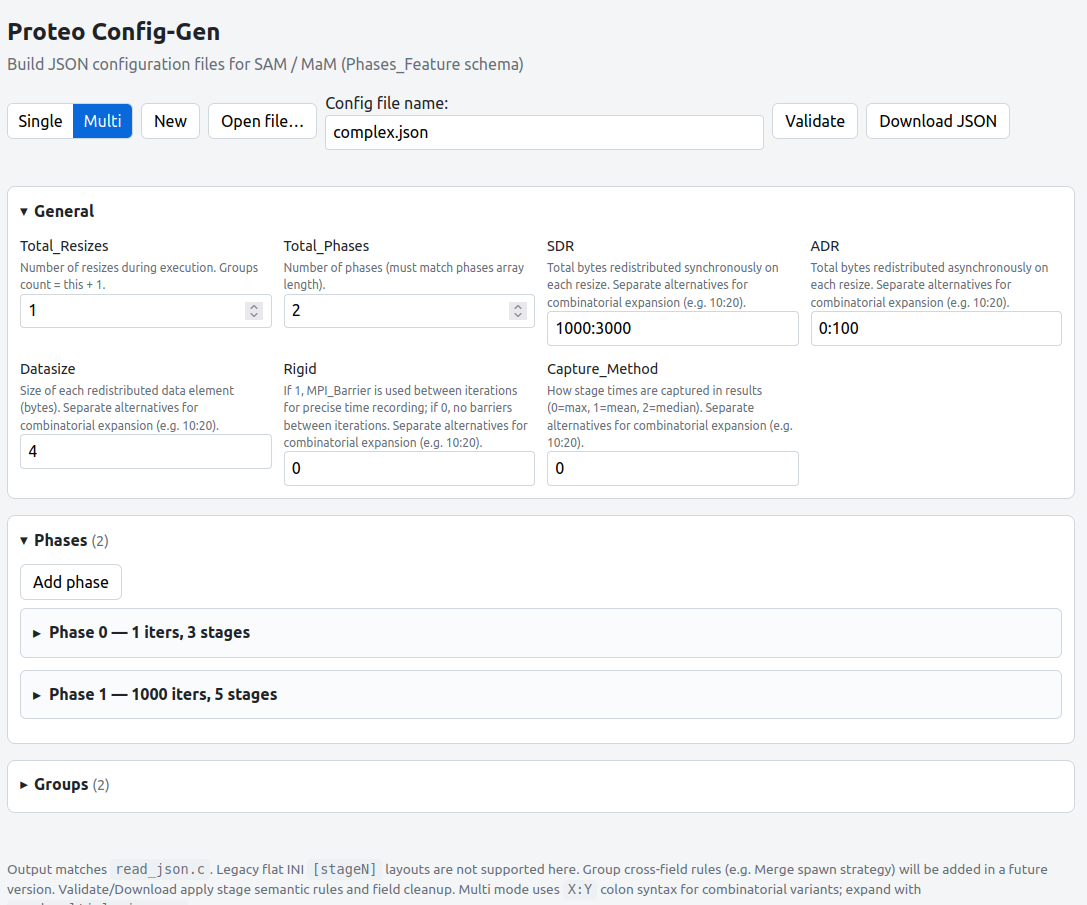
\includegraphics[width=0.95\textwidth]{GenConfig.png}
  \caption{GenConfig editor (Single mode).}
  \label{fig:genconfig-ui}
\end{figure}

\subsection{Editor workflow}

\begin{enumerate}
  \item On start, the editor loads a \textbf{minimal blank} configuration (one phase, one stage, one group).
  \item \textbf{New}: in Single mode loads a template from \texttt{Codes/test.json} when available; in Multi mode loads a blank complex scaffold.
  \item Edit \textbf{General}, \textbf{Phases} (collapsible, with nested stages), and \textbf{Groups} sections.
  \item Set \textbf{Config file name} for downloads (default \texttt{config.json} or \texttt{complex.json} in Multi mode).
  \item \textbf{Validate}: runs structural, stage, and group checks; applies field cleanup (\textit{sanitization}).
  \item \textbf{Download JSON}: saves the current configuration locally. Download is never blocked; validation messages are advisory.
  \item \textbf{Open file\ldots}: load JSON from disk; auto-detects Multi mode when variant strings contain \texttt{:}.
\end{enumerate}

Counts stay synchronized automatically:
\begin{itemize}
  \item \texttt{Total\_Phases} = number of phase cards.
  \item \texttt{Total\_Resizes} = number of groups $-$ 1.
  \item Each phase's \texttt{Total\_Stages} = number of stages in that phase.
\end{itemize}

\subsection{Single vs Multi mode}

Use the toolbar toggle \textbf{Single} | \textbf{Multi}:

\begin{description}
  \item[Single mode] Edit one concrete configuration. Numeric fields, select boxes for enums, and strategy arrays. Output is a ready-to-run JSON file for \texttt{singleRun.sh}.
  \item[Multi mode] Edit a \textbf{complex} configuration with combinatorial variants. Scalar fields accept strings such as \texttt{"10:20"}. Strategy fields accept \texttt{"0,1:0"} syntax. Validate shows how many valid expanded outputs would be produced. Download saves the complex file for CLI expansion.
\end{description}

\subsection{Combinatorial variant syntax}

\begin{table}[H]
\centering
\small
\begin{tabular}{@{}llp{6.5cm}@{}}
\toprule
\textbf{Delimiter} & \textbf{Meaning} & \textbf{Example} \\
\midrule
\texttt{:} & Cartesian alternative & e.g.\ \texttt{"500000:1000000"} yields two SDR element counts \\
\texttt{,} & Values kept together & e.g.\ \texttt{"0,1:0"} yields \texttt{[0,1]} or \texttt{[0]} \\
\bottomrule
\end{tabular}
\caption{Multi-mode variant syntax (INI-compatible convention).}
\end{table}

\textbf{Rules:}
\begin{itemize}
  \item Structural counts (\texttt{Total\_Phases}, \texttt{Total\_Resizes}, \texttt{Total\_Stages}) cannot use variants.
  \item \texttt{ADR} values 0--100 with variant \texttt{SDR} are percentages (same as legacy INI \texttt{correct\_adr}).
  \item Parallel \texttt{Procs} / \texttt{FactorS} pairs must have matching variant counts.
  \item Expansion skips combinations with duplicate consecutive \texttt{Procs} across groups.
\end{itemize}

Example complex file: \texttt{GenConfig/examples/complex.example.json}.

\subsection{Expanding complex JSON}

From the repository root:

\begin{lstlisting}[style=bashstyle,caption={CLI expansion.},captionpos=b]
python3 Exec/PythonCodes/read_multiple_json.py \
  GenConfig/examples/complex.example.json my_run_
\end{lstlisting}

Writes \texttt{Desglosed-<date>/my\_run\_0.json}, \texttt{my\_run\_1.json}, \ldots{} Each output passes structural and stage semantic validation.

Then execute any concrete file inside an existing allocation:

\begin{lstlisting}[style=bashstyle]
bash Exec/singleRunCostum.sh Desglosed-2026-07-13/my_run_0.json 0 1 0
\end{lstlisting}

\subsection{Strategy legend in the UI}

GenConfig shows spawn and redistribution strategy names (indices \textbf{1} and above; \textbf{0} means clear and is omitted from the legend):

\textbf{Spawn:} 1=Pthread, 2=Single, 3=Intercomm, 4=Multiple, 5=Parallel.

\textbf{Redistribution:} 1=Pthread, 2=Wait sources, 3=Wait targets.

Leave a strategy field empty for the default clear value \texttt{[0]}. Strategy combination constraints apply when \texttt{ADR}~$>$~0 (Section~\ref{subsubsection:strategy-rules}).

\subsection{Related files}

\begin{table}[H]
\centering
\small
\begin{tabular}{@{}ll@{}}
\toprule
\textbf{File} & \textbf{Role} \\
\midrule
\texttt{app.py} & Flask server and API endpoints \\
\texttt{schema.py} & Field metadata, enums, defaults \\
\texttt{validator.py} & Structural validation \\
\texttt{stage\_rules.py} & Stage sanitization and semantics \\
\texttt{restrictions.py} & Group cross-field rules \\
\texttt{expand\_multi.py} & Variant parsing and Cartesian expansion \\
\texttt{static/app.js} & Browser UI logic \\
\texttt{examples/complex.example.json} & Sample multi-config \\
\bottomrule
\end{tabular}
\caption{GenConfig source files.}
\end{table}

See \texttt{GenConfig/README.md} for API details (\texttt{/api/validate}, \texttt{/api/multi/preview}, etc.).

\section{Examples}
\label{section:examples}

This section walks through typical Proteo workflows with JSON configurations.

\subsection{Minimal single run}

Use the bundled test configuration \texttt{Codes/test.json} (three phases, two resizes, multiple stage types including I/O):

\begin{lstlisting}[style=bashstyle,caption={Run test.json with Slurm auto-allocation.},captionpos=b]
cd Results
bash ../Exec/singleRun.sh ../Codes/test.json mypartition 0 1 0
bash ../Exec/CheckRun.sh test 0 1 4 3 100
\end{lstlisting}

Expected outputs (index~0): \texttt{R0\_Global.out}, \texttt{R0\_G0NP2.out}, \texttt{R0\_G1NP4.out}, \texttt{R0\_G2NP6.out}, plus \texttt{slurm-*.out}.

\subsection{Custom allocation}

Obtain a Slurm allocation first, then run inside it:

\begin{lstlisting}[style=bashstyle,caption={Run inside an sbatch allocation.},captionpos=b]
sbatch -N 2 -p mypartition --wrap \
  "bash Exec/singleRunCostum.sh Codes/test.json 0 5 0"
\end{lstlisting}

This runs five repetitions with output prefix \texttt{R0}. Use a different \texttt{outIndex} (2nd argument) to distinguish batches: \texttt{R5\_*}, \texttt{R6\_*}, etc.

\subsection{Creating a config with GenConfig}

\begin{enumerate}
  \item Start GenConfig (\texttt{python3 app.py} in \texttt{GenConfig/}).
  \item Stay in \textbf{Single} mode. Click \textbf{New} to load the \texttt{test.json} template.
  \item Adjust \texttt{Procs} and \texttt{Iters} in the groups section.
  \item Click \textbf{Validate}, then \textbf{Download JSON} as \texttt{my\_experiment.json}.
  \item Inside an allocation: \texttt{bash Exec/singleRunCostum.sh my\_experiment.json 0 1 0}.
\end{enumerate}

\subsection{Simple resize example}

Listing~\ref{code:json-full-example} (Section~\ref{section:json-config}) defines one phase with Monte Carlo + Allreduce + Allgather, resizing from 2 to 10 processes after one source-group iteration. Save it as \texttt{simple\_resize.json} and run:

\begin{lstlisting}[style=bashstyle]
bash Exec/singleRunCostum.sh simple_resize.json 0 1 0
\end{lstlisting}

\subsection{Multi-phase application}

Phase~0 of \texttt{Codes/test.json} mixes I/O read, Bcast, and compute:

\begin{lstlisting}[language=json,caption={Phase 0 of Codes/test.json.},captionpos=b,label=code:json-phase-excerpt]
{
  "Total_Iters": 1,
  "Total_Stages": 3,
  "stages": [
    {
      "Stage_Type": 10,
      "Stage_Bytes": 0,
      "Stage_Involved_Procs": 2,
      "Stage_Time": 4,
      "Granularity": 1000
    },
    { "Stage_Type": 5, "Stage_Bytes": 1000, "Stage_Time": 0 },
    {
      "Stage_Type": 0,
      "Stage_Bytes": 0,
      "Stage_Time": 1,
      "Granularity": 10000
    }
  ]
}
\end{lstlisting}

Phase~1 runs 22 iterations with compute + two Allreduce stages + Allgather; phase~2 performs a single large I/O write. This illustrates how phases chain different stage sequences within the same process group.

\subsection{Combinatorial study}

Variant fields in \texttt{GenConfig/examples/complex.example.json}:

\begin{lstlisting}[language=json,caption={Variant fields in complex.example.json.},captionpos=b]
"SDR": "500000:1000000",
"ADR": "0:50",
"Procs": "2:4",
"FactorS": "1:1"
\end{lstlisting}

\textbf{Workflow:}
\begin{enumerate}
  \item Edit variants in GenConfig Multi mode (or edit the file directly).
  \item Validate to see the predicted number of valid combinations.
  \item Download as \texttt{complex.json}.
  \item Expand: \texttt{python3 Exec/PythonCodes/read\_multiple\_json.py complex.json sweep\_}.
  \item Run each \texttt{Desglosed-*/sweep\_N.json} with \texttt{singleRun.sh}, varying partition and output index as needed.
\end{enumerate}

\subsection{Conjugate-gradient-like profile}

A CG-like iteration can be approximated with one compute stage plus several communication stages (see Listing~\ref{code:json-full-example} for structure). Use matrix--vector compute (\texttt{Stage\_Type}: 1), small Allreduce messages (\texttt{Stage\_Bytes}: 8), and a large Allgather (\texttt{Stage\_Bytes} set explicitly). Tune \texttt{Granularity} and \texttt{Stage\_Time} to match target iteration time on a reference process count, then set \texttt{FactorS} per group for scaling behaviour.

\subsection{Error checking after a batch}

After multiple runs sharing prefix \texttt{exp}:

\begin{lstlisting}[style=bashstyle]
bash Exec/CheckRun.sh exp 9 5 4 3 120
\end{lstlisting}

Checks indices~0 through~9, five repetitions each, expecting four stages and three groups, rejecting iterations longer than 120~seconds.

\section{Output analysis}
\label{section:analysis}

Simulation runs produce intermediate text files (Section~\ref{subsection:intermediate_files}). This section describes the Python tooling available today for turning those files into structured data.

\subsection{Analysis scripts}

Post-processing is handled by scripts in \texttt{Analysis/}. The recommended pipeline is:

\begin{enumerate}
  \item \textbf{\texttt{MallTimes.py}}: primary entry point. Reads raw Proteo \texttt{.out} files and produces the base dataframe(s) / CSV used by downstream steps.
  \item \textbf{\texttt{joinDf.py}}: when experiments were split into multiple dataframe files, merges them into one (\texttt{python3 joinDf.py df1.pkl df2.pkl outputName}).
  \item \textbf{\texttt{CreateIterDataframe.py}}, \textbf{\texttt{CreateStageDataframe.py}}, \textbf{\texttt{CreateResizeDataframe.py}}: derive specialised views (per-iteration, per-stage, per-resize) from the MallTimes output.
\end{enumerate}

Example:

\begin{lstlisting}[style=bashstyle,caption={Build base dataframe from result files.},captionpos=b]
python3 Analysis/MallTimes.py R /path/to/results/ data_global.csv
\end{lstlisting}

\begin{description}
  \item[\texttt{R}] Common prefix of Proteo output files (e.g.\ \texttt{R} matches \texttt{R0\_Global.out}, \texttt{R1\_Global.out}, \ldots).
  \item[\texttt{/path/to/results/}] Directory containing result subdirectories or flat output files.
  \item[\texttt{data\_global.csv}] Output path for the aggregated data.
\end{description}

\textbf{Requirements:} Python~3 with NumPy and Pandas.

\subsection{Notebook analyser (WIP)}

\texttt{Analysis/new\_analyser.ipynb} is a work-in-progress Jupyter notebook for statistical summaries and plots. It is \textbf{not yet suitable for general use} by other users (hard-coded paths, evolving API). Future manual revisions will document it once stabilised.

\subsection{Recommended practice}

\begin{itemize}
  \item Run \texttt{CheckRun.sh} before analysis to filter or relaunch inconsistent repetitions.
  \item Use at least five repetitions per configuration when comparing strategies statistically.
  \item Keep \texttt{Rigid=1} when precise iteration timing matters; use \texttt{Rigid=0} for performance-oriented studies where barrier overhead should be avoided.
\end{itemize}

For column-level CSV documentation, see Appendix~\ref{appendix:csv}.


\appendix
\section{Output CSV files format}
\label{appendix:csv}

In this appendix is described the format of each final output file, in order to allow users to analyze by themselves the obtained results.

Each of the rows of file \textit{data\_global.csv} represents a complete execution of a malleable application. Columns can be grouped according to their meaning. On the one hand, there are those showing information on the resizing, on the computation in each iteration and the results obtained.
%The first data set \textit{data\_global.csv}, where each row represents a whole execution, has the next columns types:
\begin{itemize}
    \item Columns related to resize configuration:
    \begin{itemize}
        \item Total\_Resizes: It is an integer that indicates number of performed resizes (\texttt{Total\_Resizes} in configuration file). %Integer.
        \item Total\_Groups: It is an integer indicating the number of processes groups for the malleable execution. It is equal to \texttt{Total\_Resizes}$+1$.% Integer.
        Each of the following six columns is a list of data showing the concrete information for each group in a resize. They are a ordered array of integers with size \textit{Total\_Groups}.  
        \item Groups: Number of processes in a group. %of executed processes group during the execution of malleable application. Array of integers with size \textit{Total\_Groups}.
        \item Dist: Physical distribution of processes in a group. %Array of integers with size \textit{Total\_Groups}. 
        Its possible values are Compact(0) and Spread(1).
        \item Spawn\_Method: Spawn method for a resize.% Array of integers with size \textit{Total\_Resizes}. 
        Its possible values are Baseline(0) and Merge(1).
        \item Spawn\_Strategy: Spawn strategy for a resize. %Array of integers with size \textit{Total\_Resizes}. 
        Its possible values are None(1), Single(3), Asynchronous(2) and All(6).
        \item Redistribution\_Method: Redistribution method for each resize. Array of integers with size \textit{Total\_Groups}. Its possible values are Alltoall (0), Point-to-point(1), RMA-Lock(2) or RMA-LockAll(3).
        \item Redistribution\_Strategy: Redistribution strategy for each resize. Array of integers with size \textit{Total\_Groups}. Its possible values are None(1), Threads(2).
        \item SDR: Number of data elements redistributed synchronously in each redistribution stage. Integer. Multiply by \texttt{Datasize} for bytes moved.
        \item ADR: Number of data elements redistributed asynchronously in each redistribution stage. Integer. Multiply by \texttt{Datasize} for bytes moved.
        \item DR: Total elements redistributed in each redistribution stage. Is equal to $SDR + ADR$. Integer.
    \end{itemize}
    
    \item Columns related to application type: %compute configuration:
    \begin{itemize}
        \item Granularity: It is an integer that indicates problem size for computation stages. %Integer.
        \item FactorS: Speedup factor to emulate how the performance of computation stages are affected by the number of processes. Ordered array of Integers of size \textit{Total\_Groups}.
        \item Total\_Stages: It is an integer that represents number of stages in an iteration. The three following columns contain concrete information about each of stages. They will be an ordered array of size \textit{Total\_Stages}.
        \item Stage\_Types: Each element indicates stage type (computation/communication). %Ordered array of stage types for each stage of the iterations. Array of integers with size \textit{Total\_Stages}.
        Its possible values are PI\_Computation(0), Matrix\_Computation(1), Point\_communication(2), Bcast\_communication(3), Allgatherv\_communication(4), Reduce\_communication(5) and Allreduce\_communication(6).
        \item Stage\_Times: Each element represents the stage time. %for each stage of the iterations. Array of integers with size \textit{Total\_Stages}.
        \item Stage\_Bytes: Each element indicates bytes communicated in this stage. %for each stage of the iterations. Array of integers with size \textit{Total\_Stages}.
        For computation stages is always 0.
        %\item $Latency_{net}$: Latency of the used network.
        %\item $Bw_{net}$: Bandwidth of the used network.
        %\item $Latency_{shm}$: Latency of the used shared memory.
        %\item $Bw_{shm}$: Bandwidth of the used shared memory.
    \end{itemize}
    
    \item Results columns:
    \begin{itemize}
        \item Iters:  It is an  ordered array of integers with size \textit{Total\_Groups} that contains  executed iterations by each group. % Is the sum of \textit{Asynch\_Iters} and synchronous iterations. %Array of integers with size \textit{Total\_Groups}.
        \item Asynch\_Iters: It is an ordered array of integers with size \textit{Total\_Groups} that represents the total iterations executed  by the parents while an asynchronous resize was taking place. %Array of integers with size \textit{Total\_Resizes}.
        \item $T_{iter}$: Array of arrays (2 levels) which contains the times of each  iteration. The upper array refers to the iterations of each group and has a size of \textit{Total\_Groups}. The inner array contains floats, and the size of the array with index \textit{i} is \textit{Iters[i]}, where \textit{i} refers to a group of processes. 
        Therefore, to check the iteration time of the last iteration in the first group of processes it will be accessed as $T_{iter}[0][Iters[0]-1]$.
        \item $T_{stages}$: Array of 3 levels which contains the times of each performed stage in the execution. The first level contains arrays of groups and is of size \textit{Total\_Groups}. The second level contains an array of iterations, and the size of the array with index \textit{i} is \textit{Iters[i]}, where \textit{i} refers to a group of processes. Lastly, the third level stores for a specific iteration, an array of floats values where each one represents the time of a stage in the iteration. Has a size of \textit{Total\_Stages}.
        Therefore, to check the stage time of the last stage in the last iteration of the first group of processes it will be accessed as $T_{iter}[0][Iters[0]-1][Total\_Stages-1]$.
        
        \item $T_{spawn}$: Ordered array of spawn times for each resize. Refers to the time $T_{spawn}$ in the monitoring module (Subsection \ref{subsection:monitoring}). Array of floats with size \textit{Total\_Resizes}. 
        \item $T_{spawn\_real}$: Ordered array of real spawn times for each resize. Refers to the time $T_{spawn\_real}$ in the monitoring module (Subsection \ref{subsection:monitoring}). Array of floats with size \textit{Total\_Resizes}.
        \item $T_{SR}$: Ordered array of synchronous data redistribution times for each resize. Refers to the time $T_{SR}$ in the monitoring module (Subsection \ref{subsection:monitoring}). Array of floats with size \textit{Total\_Resizes}. 
        \item $T_{AR}$: Ordered array of asynchronous data redistributions times for each resize. Refers to the time $T_{AR}$ in the monitoring module (Subsection \ref{subsection:monitoring}). Array of floats with size \textit{Total\_Resizes}. 
        \item $T_{total}$: Total execution time of the application. Float value.
    \end{itemize}
    
\end{itemize}
The other two files generated by \textit{analyser.sh} script, \textit{data\_malleability.csv} and \textit{data\_iterations.csv}, are focused on helping the analysis of behaviour of malleable application   while resizing is being performed above  when it is carried out asynchronously. In both files, each row represents a different malleable running and its columns are a subset of those described in the previous file.

The second data set \textit{data\_malleability.csv}, is intended to facilitate the analysis of different configurations in malleability only, where all the execution data is not needed. Each row represents a single resize.
This data set has the next columns:
\begin{itemize}
    \item Resize configuration columns:
    \begin{itemize}
        \item NP: Number of parent processes before the resize. Integer.
        \item NC: Number of children processes after the resize. Integer.
        \item Dist: Physical distribution of processes for the parents and children. Array of two integers. Its possible values are Compact(0) and Spread(1).
        \item Spawn\_Method: Spawn method used for the resize. Integer. Its possible values are Baseline(0) and Merge(1).
        \item Spawn\_Strategy: Spawn strategy used for the resize. Integer. Its possible values are None(0), Asynchronous(1), Single(2), All(3).
        \item Redistribution\_Method: Redistribution method for each resize. Integer. Its possible values are Alltoall (0), Point-to-point(1), RMA-Lock(2) or RMA-LockAll(3).
        \item Redistribution\_Strategy: Redistribution strategy for each resize. Integer. Its possible values are None(1), Threads(2).
        \item SDR: Number of data elements redistributed synchronously in the redistribution stage. Integer. Multiply by \texttt{Datasize} for bytes moved.
        \item ADR: Number of data elements redistributed asynchronously in the redistribution stage. Integer. Multiply by \texttt{Datasize} for bytes moved.
        \item DR: Total elements redistributed in the redistribution stage. Is equal to $SDR + ADR$. Integer.
    \end{itemize}
    
    \item Compute configuration columns:
    \begin{itemize}
        \item Total\_Stages: Number of stages. Integer.
        \item Granularity: Problem size for computation stages. Integer.
        \item FactorS: Speedup factor to emulate how the performance of computation stages are affected by the number of processes at column \textit{NP}. Integer.
        \item Stage\_Type: Ordered array of stages types for each stage of the iterations. Array of integer with size \textit{Total\_Stages}. Its possible values are PI\_Computation(0), Matrix\_Computation(1), Point\_communication(2), Bcast\_communication(3), Allgatherv\_communication(4), Reduce\_communication(5) and Allreduce\_communication(6).
        \item Stage\_Time: Ordered array of stage times for each stage of the iterations. Array of integer with size \textit{Total\_Stages}.
        \item Stage\_Bytes: Ordered array of bytes communicated for each stage of the iterations. Array of integer with size \textit{Total\_Stages}.
        %\item $Latency_{net}$: Latency of the used network.
        %\item $Bw_{net}$: Bandwidth of the used network.
        %\item $Latency_{shm}$: Latency of the used shared memory.
        %\item $Bw_{shm}$: Bandwidth of the used shared memory.
    \end{itemize}
    
    \item Results columns:
    \begin{itemize}
        \item Iters: Quantity of performed iterations by the parents. Is the sum of \textit{Asynch\_Iters} and synchronous iterations. Integer.
        \item Asynch\_Iters: Quantity of performed iterations by the parents while an asynchronous resize was taking place. Integer.
        \item $T_{iter}$: Array of times for each performed iteration in this group. The array contains floats and has a size of \textit{Iters} elements. 
        Therefore, to check the iteration time of the last iteration it will be accessed as $T_{iter}[Iters-1]$.
        \item $T_{stages}$: Array of 2 levels which contains the times of each performed stage by the group. The first level contains an array of iterations, with an array size of \textit{Iters}. On the other hand, the second level stores for a specific iteration, an array of floats values where each one represents the time of a stage in the iteration. Has a size of \textit{Total\_Stages}.
        Therefore, to check the stage time of the last stage in the last iteration it will be accessed as $T_{stages}[Iters-1][Total\_Stages-1]$.
        
        \item $T_{spawn}$: Spawn times for the resize. Refers to the time $T_{spawn}$ in the monitoring module (Subsection \ref{subsection:monitoring}). Float value.
        \item $T_{spawn\_real}$: Real spawn times for the resize. Refers to the time $T_{spawn\_real}$ in the monitoring module (Subsection \ref{subsection:monitoring}). Float value.
        \item $T_{SR}$: Synchronous data redistribution time for the resize. Refers to the time $T_{SR}$ in the monitoring module (Subsection \ref{subsection:monitoring}). Float value.
        \item $T_{AR}$: Asynchronous data redistribution time for the resize. Refers to the time $T_{AR}$ in the monitoring module (Subsection \ref{subsection:monitoring}). Float value.
    \end{itemize}
\end{itemize}

The final data set \textit{data\_iterations.csv} is a simplification of the previous data sets to focus an analysis on how each iteration has been performed. Each row represents a single iteration.
This data set has the next columns:
\begin{itemize}
    \item NP: Number of processes. Integer.
    \item Is\_Dynamic: Whether the group of processes is the first one (False) or has been spawned during execution (True). Boolean.
    
    \item The next values should be ignored if $Asynch\_Iters$ is False. Resize configuration columns:
    \begin{itemize}
        \item NC: Number of children processes after the resize. Integer. Default value is \textit{None} if $Asynch\_Iters$ is False.
        \item Dist: Physical distribution of processes for the parents and children. Array of two integers. Its valid values are Compact(0) and Spread(1). Default value for second element is (-1) if $Asynch\_Iters$ is False.
        \item Spawn\_Method: Spawn method used for this group and the next one. Array of two integers. Its possible values are Baseline(0) and Merge(1). Default value for first element is (0) if $Is\_Dynamic$ is False. Default value for second element is (-1) if $Asynch\_Iters$ is False.
        \item Spawn\_Strategies: Spawn strategy used for this group and the next one. Array of two integers. Its possible values are None(0), Asynchronous(1), Single(2), All(3). Default value for first element is (1) if $Is\_Dynamic$ is False. Default value for second element is (-1) if $Asynch\_Iters$ is False.
        \item Redistribution\_Method: Redistribution method used for this group and the next one. Array of two integers. Its possible values are Alltoall (0), Point-to-point(1), RMA-Lock(2) or RMA-LockAll(3). Default value for first element is (0) if $Is\_Dynamic$ is False. Default value for second element is (-1) if $Asynch\_Iters$ is False.
        \item Redistribution\_Strategy: Redistribution strategy used for this group and the next one. Array of two integers. Its possible values are None(1), Threads(2). Default value for first element is (1) if $Is\_Dynamic$ is False. Default value for second element is (-1) if $Asynch\_Iters$ is False.
        \item SDR: Number of data elements redistributed synchronously in the redistribution stage. Integer. Default value is (-1) if $Asynch\_Iters$ is False.
        \item ADR: Number of data elements redistributed asynchronously in the redistribution stage. Integer. Default value is (-1) if $Asynch\_Iters$ is False.
        \item DR: Total elements redistributed in the redistribution stage. Integer. Is equal to $SDR + ADR$. Default value is (-1) if $Asynch\_Iters$ is False.
    \end{itemize}
    
    \item Compute configuration columns:
    \begin{itemize}
        \item Total\_Stages: Number of stages. Integer.
        \item Granularity: Problem size for computation stages. Integer.
        \item FactorS: Speedup factor to emulate how the performance of computation stages are affected by the number of processes at column \textit{NP}. Integer.
        \item Stages\_Type: Ordered array of stage types for each stage of the iterations. Array of integer with size \textit{Total\_Stages}. Its possible values are PI\_Computation(0), Matrix\_Computation(1), Point\_communication(2), Bcast\_communication(3), Allgatherv\_communication(4), Reduce\_communication(5) and Allreduce\_communication(6).
        \item Stage\_Time: Ordered array of stage times for each stage of the iterations. Array of integer with size \textit{Total\_Stages}.
        \item Stage\_Bytes: Ordered array of bytes communicated for each stage of the iterations. Array of integer with size \textit{Total\_Stages}.
        %\item $Latency_{net}$: Latency of the used network.
        %\item $Bw_{net}$: Bandwidth of the used network.
        %\item $Latency_{shm}$: Latency of the shared memory.
        %\item $Bw_{shm}$: Bandwidth of the used shared memory.
    \end{itemize}
    
    \item Results columns:
    \begin{itemize}
        \item $Asynch\_Iters$: Indicates whether this iteration has been performed normally (False) or during an asynchronous resize (True). Boolean.
        \item $T_{iter}$: Iteration time. Float value
        \item $T_{stage}$: Array of each stage time in the iteration. Array of floats with size \textit{Total\_Stages}. Therefore, to check the stage time of the last stage in the iteration it will be accessed as $T_{stages}[Total\_Stages-1]$.
    \end{itemize}
\end{itemize}

\end{document}
